\section{Improvements}

\begin{frame}
    \frametitle{SIFT Features}
    \begin{itemize}
        \item Extract SIFT features from image samples.
        \item Problem: How to combine different numbers of SIFT descriptors for each sample?
            \begin{itemize}
                \item Sample 1 may have 3 descriptors.
                \item Sample 2 may have 2 descriptors.
                \item Recall that an SVM requires all feature vectors to have the same length.
            \end{itemize}
        \item Shelved this idea for now, but I'm curious about tracking via SIFT over the entire
            frame.
    \end{itemize}
\end{frame}

\begin{frame}
    \frametitle{Loss Function}
    \begin{itemize}
        \item Existing loss function is based on bounding box overlap.
        \item Add a loss function based on translation distance.
            \begin{align}
                \Delta \left( \mathbf{y}, \mathbf{\bar{y}} \right) &= \frac{\|\mathbf{y} -
                \mathbf{\bar{y}}\|}{d_{max}} \\ \nonumber \\
                d_{max} &= \sqrt{h_{image}^2 + w_{image}^2}
            \end{align}
    \end{itemize}
\end{frame}

\begin{frame}
    \frametitle{Loss Function}
    Todo: Add images visualizing the loss functions.
\end{frame}

\begin{frame}
    \frametitle{Loss Manipulation}
    \begin{columns}[T]
        \begin{column}{0.5\textwidth}
            \begin{itemize}
                \item Original Struck did not allow shaping the loss function.
                \item Added a loss manipulator:
                    \begin{equation}
                        f(\Delta) = 3\Delta^2 - 2\Delta^3 : \Delta \in [0, 1]
                    \end{equation}
            \end{itemize}
        \end{column}
        \begin{column}{0.5\textwidth}
            \includegraphics[height=0.8\textheight]{loss_manipulator}
        \end{column}
    \end{columns}
\end{frame}

\begin{frame}
    \frametitle{Weighted Struck}
    \begin{itemize}
        \item Add a scalar weight.
            \begin{align}
                F\left(\mathbf{x}, \mathbf{y}\right) &= \sum_{i, \mathbf{\bar{y}}} \beta_i^\mathbf{\bar{y}}
                    \langle \kappa\left(\mathbf{x}_i, \mathbf{\bar{y}}\right),
                    \kappa\left(\mathbf{x}, \mathbf{y}\right) \rangle
                    \tag{\ref{eq:discriminant_function}} \\
                F\left(\mathbf{x}, \mathbf{y}\right) &= \alert{s(\mathbf{y})} \sum_{i, \mathbf{\bar{y}}} \beta_i^\mathbf{\bar{y}}
                    \langle \kappa\left(\mathbf{x}_i, \mathbf{\bar{y}}\right),
                    \kappa\left(\mathbf{x}, \mathbf{y}\right) \rangle
            \end{align}
    \end{itemize}
\end{frame}

\begin{frame}
    \frametitle{Weight function}
    \begin{align}
        s \left( \mathbf{y} \right) &= \frac{\|\mathbf{y}\|}{d_{max}} \\
        \nonumber \\
        d_{max} &= \sqrt{h_{image}^2 + w_{image}^2}
    \end{align}
\end{frame}

\begin{frame}
    \frametitle{Sampling locations - Weighted Struck}
    \begin{columns}
        \begin{column}{0.5\textwidth}
            Original Struck

            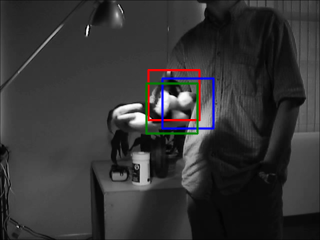
\includegraphics[width=\textwidth]{sylv}
        \end{column}
        \begin{column}{0.5\textwidth}
            Weighted Struck

            \includegraphics[width=\textwidth]{sylv_fuzzy}
        \end{column}
    \end{columns}
\end{frame}

